   \documentclass{article}

%other packages
\usepackage[a4paper,paperwidth=5in,paperheight=3.7in]{geometry}
\usepackage{longtable}
\usepackage{wrapfig}
\setlength\parindent{0pt}
\usepackage{enumitem}
\usepackage[table]{xcolor}
\usepackage{polynom}
\def\scaleint#1{\vcenter{\hbox{\scaleto[3ex]{\displaystyle\int}{#1}}}}
\usepackage{array}
\newcolumntype{C}{>{{}}c<{{}}} % for '+' and '-' symbols
\newcolumntype{R}{>{\displaystyle}r} % automatic display-style math mode 
\usepackage{tabularray}
\usepackage{dcolumn,tabularx,booktabs}
\usepackage{esvect}
\usepackage{nopageno}

%maths
\usepackage{mathtools}
\usepackage{amsmath}
\usepackage{amssymb}
\usepackage{amsfonts}
\usepackage{autobreak}

%tikzpicture
\usepackage{tikz}
\usepackage{scalerel}
\usepackage{pict2e}
\usepackage{tkz-euclide}
\usepackage{tikz-3dplot}
\usetikzlibrary{calc}
\usetikzlibrary{patterns,arrows.meta}
\usetikzlibrary{shadows}
\usetikzlibrary{external}
\usetikzlibrary{decorations.pathreplacing,angles,quotes}
\usetikzlibrary{perspective,spath3}

%pgfplots
\usepackage{pgfplots}
\pgfplotsset{compat=1.18}
\usepgfplotslibrary{statistics}
\usepgfplotslibrary{fillbetween}

\pgfplotsset{
    standard/.style={
    axis line style = thick,
    trig format=rad,
    enlargelimits,
    axis x line=middle,
    axis y line=middle,
    enlarge x limits=0.15,
    enlarge y limits=0.15,
    every axis x label/.style={at={(current axis.right of origin)},anchor=north west},
    every axis y label/.style={at={(current axis.above origin)},anchor=south east}
    }
}

\begin{document}
 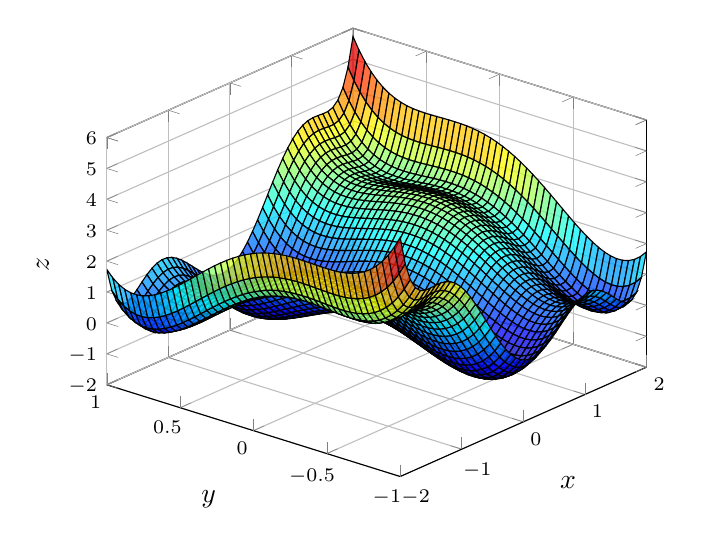
\begin{tikzpicture}
        \begin{axis}[
        align =center,
        view={310}{30},
        xtick = {2,1,...,-2},
        ytick = {1,0.5,...,-1},
        ztick = {6,5,...,-2},
        xmin=-2,
        xmax=2,
        ymin=-1,
        ymax=1,
        zmin=-2,
        zmax=6,
        ticklabel style = {font = \scriptsize},
        grid=major,
        xlabel=$x$,
        ylabel=$y$,
        zlabel=$z$      
            ]

            \addplot3 [
                surf,
            shader = flat,
            draw = black,
                colormap/jet,
                %shader=faceted,
                fill opacity=0.75,
                samples=50,
                domain=-2:2,
                y domain=-1:1
                ] {(4-2.1*x^2+x^4/3)*x^2+x*y+(-4+4*y^2)*y^2};

        \end{axis}
   \end{tikzpicture} 
\end{document}